\documentclass[10pt]{scrartcl}
\usepackage{graphicx}
\usepackage{float}
\usepackage{amsmath}
\usepackage[utf8]{inputenc} 
\usepackage[T1]{fontenc}
\usepackage{lmodern}
\usepackage{amsfonts}   
\usepackage{amssymb}
\usepackage{mathtools}
\usepackage{epstopdf}
\usepackage[shadow]{todonotes}

 
\begin{document}

\title{Dokumentation zum Java Code Camp 21.02.2020}

%Bitte hier Namen Pflegen!
\author{Christian Küllmer, Gianluca Voss}
\date{\today{}, Kassel}
\maketitle
\begin{figure}[H]
	\centering
	
\includegraphics[width=0.6\textwidth]{Bilder/Titelblatt/big_logo.png}
\end{figure}
\todo{Bitte pflegt eure Namen auf dieser Seite!}
\newpage
%Inhaltsverzeichnis
\renewcommand{\contentsname}{Inhaltsverzeichnis}
\tableofcontents
\newpage
%Ab hier bitte neuen Stuff von euch pflegen!

\section{Überblick}
%In diesem Abschnitt bitte nur einen Überblick über die Ziele dieses Projekts geben!

In diesem Abschnitt werden die Gedanken, welche bei der Entstehung der App getätigt wurden, erläutert. Man findet hier die Erläuterungen um die einzelnen Gedankengänge beim Entstehen der App nach zu vollziehen und das Gesamprodukt richtig einordnen zu können.

\subsection{Worum geht es in der App Broken Broke Broker}
In der App "Broken Broke Broker" geht es um die Simulation einer Börsenumgebung in der, der Nutzer einzelne Wertpapiere, Währungen oder Kryptowährungen kaufen kann. Auf dem Smartphone wird ein Spiel begonnen indem es um den Handel mit Wertpapieren geht. Die Kursdaten werden dabei aus dem Web gezogen. Die App soll in Java geschrieben werden und die einzelnen Anwendungen sollen möglichst intuitiv von dem Benutzer zu bedienen sein. Die Menüführung soll klar strukturiert und in einem Stil sein, der es möglich macht sich voll auf den Handel mit Devisen und Wertpapieren zu konzentrieren.

\subsubsection{Anforderungen}
Folgende Features sollen mir der oben gewählten Technologie umgesetzt werden:

Bei der oben gewählten Technologie sollen die im Folgenden vorgestellten Hauptfunktionen zur Verfügung gestellt werden.

\begin{enumerate}
	\item 
	Suche nach Aktien, Währungen, Digitalwährungen
	\item
	Anlegung eines Portfolios
	\item
	Übersicht über Depot, Kontostand und Verlauf
	\item
	Darstellung der aktuellen Kurse als Graph
	\item
	Aktien kaufen / verkaufen
	\item
	Transaktionskosten
	\item
	Historie über Käufe / Verkäufe
	\item
	Kaufoption / Verkaufsoption
	\item
	Hintergrundservice für Kauf- / Verkaufsaufträge
	\item
	Spiel zurücksetzen / neustarten
\end{enumerate}


Zu den Hauptfunktionen wurde die Forderung gestellt, dass alle funktionieren müssen. Des Weiteren soll eine Zusatzfunktion implementiert werden und es muss die Stabilität der Applikation gewährleistet sein, darf folglich nicht abstürzen. Eine Dokumentation, sowie eine Präsentation wurde gefordert. Aufgrund der Verbreitung des Coronavirus, wurde hierbei von der Präsentation abgesehen.



\subsection{Motivation}
%In diesem Abschnitt bitte nur beschreiben, wie die Zielvorstellung aussieht.
Die Motivation für uns bei diesem Code Camp die App in Java zu schreiben liegt vor allem darin sich als Team einer unbekannten Herausforderung zu stellen. Eine Herausforderung an deren Ende ein Programm steht, welches Spaß beim Spielen macht und einen Einblick in die Welt des Finanzmarktes gibt. Die App heißt Broken Broke Borker um die Tatsache zu verdeutlichen, dass es um 

\subsection{Herangehensweise}
%Wir die einzelnen Ziele erreicht werden sollten werden wir in diesem Abschnitt hinterlegen!

\section{Funktionalität der Applikation}
%Beschreiben der einzelnen GUI Oberflächen und deren Funktion. 
%Bitte selbstständig die einzlenen Abschnitte mit den Screens ergänzen!


\subsection{Technische Details}

\subsection{Verwendete Programmierbibliotheken}

\begin{enumerate}
	
	\item 
	AnyChart Android

\begin{figure}[H]
	\centering
	
\includegraphics[width=0.6\textwidth]{Bilder/BibliothekenLogos/Anychart.png}
\end{figure}

% link: https://www.anychart.com/blog/wp-content/uploads/2016/05/AnyChart_JS_HTML5_Charts_Maps_Stock_Graphs_Dashboards_logo_300x92.png

AnyChart ist eine leichte und robuste JavaScript-Diagrammbibliothek mit hervorragender API, Dokumentation und Unterstützung für Unternehmen.

Es wurde seit 2003 mit einer Hauptidee entwickelt: Es sollte für jeden Entwickler einfach sein, schöne Diagramme in jedes mobile, Desktop- oder Webprodukt zu integrieren. Daher ist AnyChart heute eine Datenvisualisierungsschicht für Tausende großartiger Produkte. Unseres gehört nun auch dazu, wenn auch nur mit der Trial Version.


	\item 
	OkHttpClient

\begin{figure}[H]
	\centering
	
\includegraphics[width=0.6\textwidth]{Bilder/BibliothekenLogos/OKHTTP.jpg}
\end{figure}

% link: https://duckduckgo.com/?q=okhttpclient+logo&iax=images&ia=images&iai=https%3A%2F%2Fwww.mkyong.com%2Fwp-content%2Fuploads%2F2019%2F10%2FOkHttp-logo.png

HTTP ist das moderne Anwendungsnetzwerk. So tauschen wir Daten und Medien aus. Durch effizientes Ausführen von HTTP werden Inhalte schneller geladen und Bandbreite gespart.

OkHttp ist ein HTTP-Client, der standardmäßig effizient ist:

Durch die HTTP / 2-Unterstützung können alle Anforderungen an denselben Host einen Socket gemeinsam nutzen.
Das Verbindungspooling reduziert die Anforderungslatenz (wenn HTTP / 2 nicht verfügbar ist).
Transparentes GZIP verkleinert die Downloadgröße.
Durch das Zwischenspeichern von Antworten wird das Netzwerk für wiederholte Anforderungen vollständig vermieden.
OkHttp bleibt bestehen, wenn das Netzwerk Probleme hat: Es wird stillschweigend von häufigen Verbindungsproblemen wiederhergestellt. Wenn der Dienst mehrere IP-Adressen hat, versucht OkHttp, alternative Adressen zu finden, wenn die erste Verbindung fehlschlägt. Dies ist für IPv4 + IPv6 und Dienste erforderlich, die in redundanten Rechenzentren gehostet werden. OkHttp unterstützt moderne TLS-Funktionen (TLS 1.3, ALPN, Pinning von Zertifikaten). Es kann so konfiguriert werden, dass es auf eine breite Konnektivität zurückgreift.

Die Verwendung von OkHttp ist einfach. Die Anforderungs- / Antwort-API wurde mit fließenden Buildern und Unveränderlichkeit entwickelt. Es unterstützt sowohl synchron blockierende calls als auch asynchrone calls mit callback.


	\item
	JSON.simple
	
\begin{figure}[H]
	\centering
	
\includegraphics[width=0.6\textwidth]{Bilder/BibliothekenLogos/JSONLogo.png}
\end{figure}

% link: http://aommaster.com/blog/wp-content/uploads/2015/10/JSONLogo.png
	
JSON.simple ist ein einfaches Java-basiertes Toolkit für JSON. Mit JSON.simple kann man JSON-Daten codieren oder decodieren.

	\item
	Android Maerial Components
	
\begin{figure}[H]
	\centering
	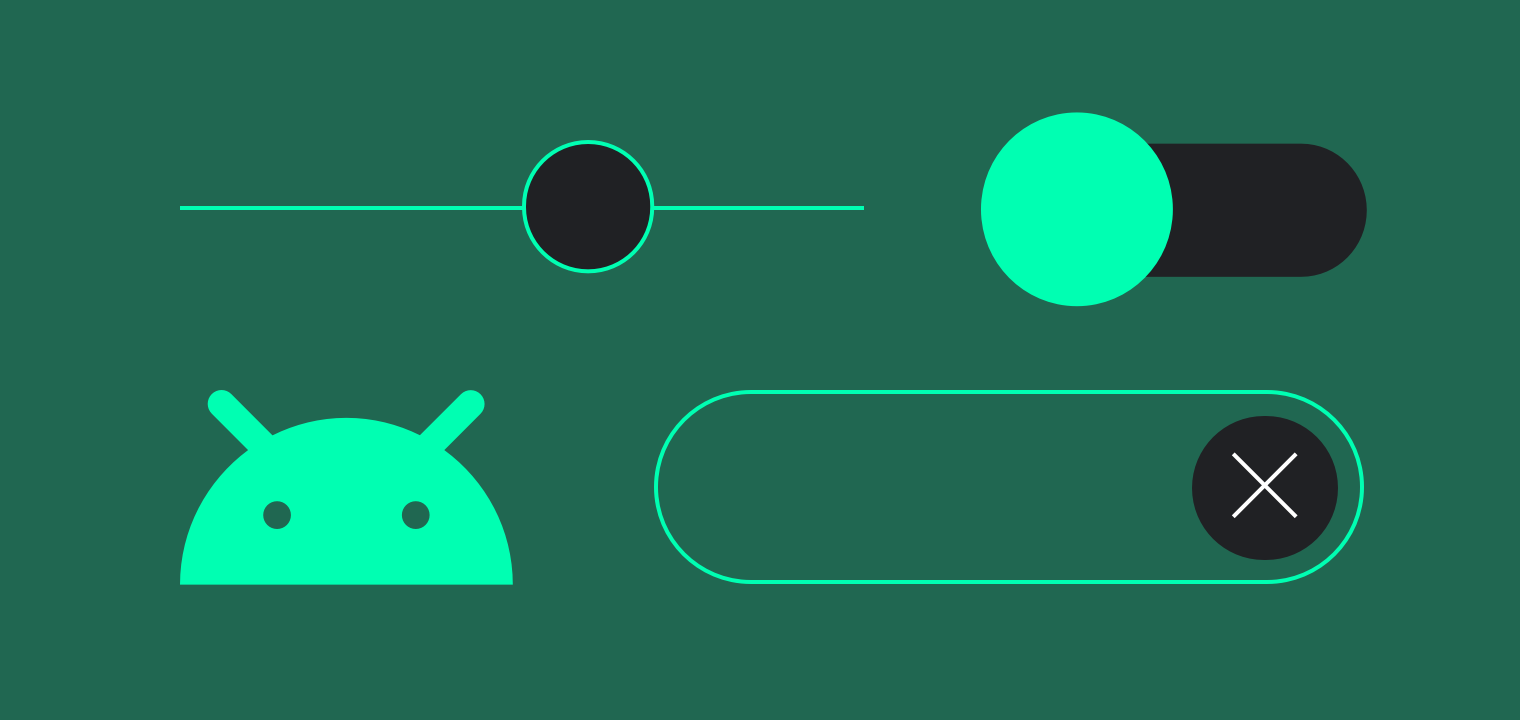
\includegraphics[width=0.6\textwidth]{Bilder/BibliothekenLogos/AndroidMaterialComponenLogo.png}
\end{figure}


% link: https://material.io/develop/assets/1kvhm0FosmH_nzjOHdtnFX3dQObsxnjv_/android-documents-how-to-components-2x1-large.png

Material Components für Android (MDC-Android) unterstützt Entwickler bei der Ausführung von Material Design. Diese Komponenten wurden von einem Kernteam aus Ingenieuren und UX-Designern bei Google entwickelt und ermöglichen einen zuverlässigen Entwicklungsworkflow zum Erstellen schöner und funktionaler Android-Apps.

Material Components für Android ist ein Ersatz für die Design Support Library von Android.

	\item
	Androidx

\begin{figure}[H]
	\centering
	
\includegraphics[width=0.6\textwidth]{Bilder/BibliothekenLogos/AndroidLogo.png}
\end{figure}
	
% link: https://upload.wikimedia.org/wikipedia/commons/thumb/d/d7/Android_robot.svg/1200px-Android_robot.svg.png

Artefakte im Androidx-Namespace umfassen die Android Jetpack-Bibliotheken. Wie die Support-Bibliothek werden Bibliotheken im theandroidx namespace separat von der Android-Plattform geliefert und bieten Abwärtskompatibilität für alle Android-Versionen.

AndroidX ist eine wesentliche Verbesserung gegenüber der ursprünglichen Android-Support-Bibliothek, die nicht mehr gepflegt wird. AndroidX-Pakete ersetzen die Support-Bibliothek vollständig, indem sie Feature-Parität und neue Bibliotheken bereitstellen.

\end{enumerate}


\subsection{Navigationsschema zwischen den Bildschirmen}

Navigation
Alle Hauptseiten sind durch die Navigation verbunden. Bei jeder Hauptseite befindet sich am Oberen Ende des Bildschirms eine Leiste, in der sich der Name der aktuellen Seite, sowie rechts ein Suchsymbol und  links ein Menüzeichen, mit der sich die Navigation öffnen lässt, befindet. Durch Öffnen der Navigation verlässt man nicht seine aktuelle Seite, sondern sie legt sich von der linken Seite des Geräts über zwei Drittel des Bildschirms und verdunkelt das restliche Drittel leicht. 
Oben in der Navigation ist das Logo der Applikation, ein buntes "Broken Broke Broker", zu sehen. Darunter sind nacheinander die Hauptseiten aufgelistet. Jede Seite hat in seiner Reihe ein zu der Funktion passendes Symbol erhalten und ist erreichbar, indem man auf die genante Reihe drückt. Die Navigation schließt sich, wenn man entweder auf eine der aufgelisteten Seiten oder in das rechte Drittel klickt. Bei ersterem wird zu der Seite navigiert und bei späterem bleibt man einfach auf der aktuellen Seite.

\begin{figure}[H]
	\centering
	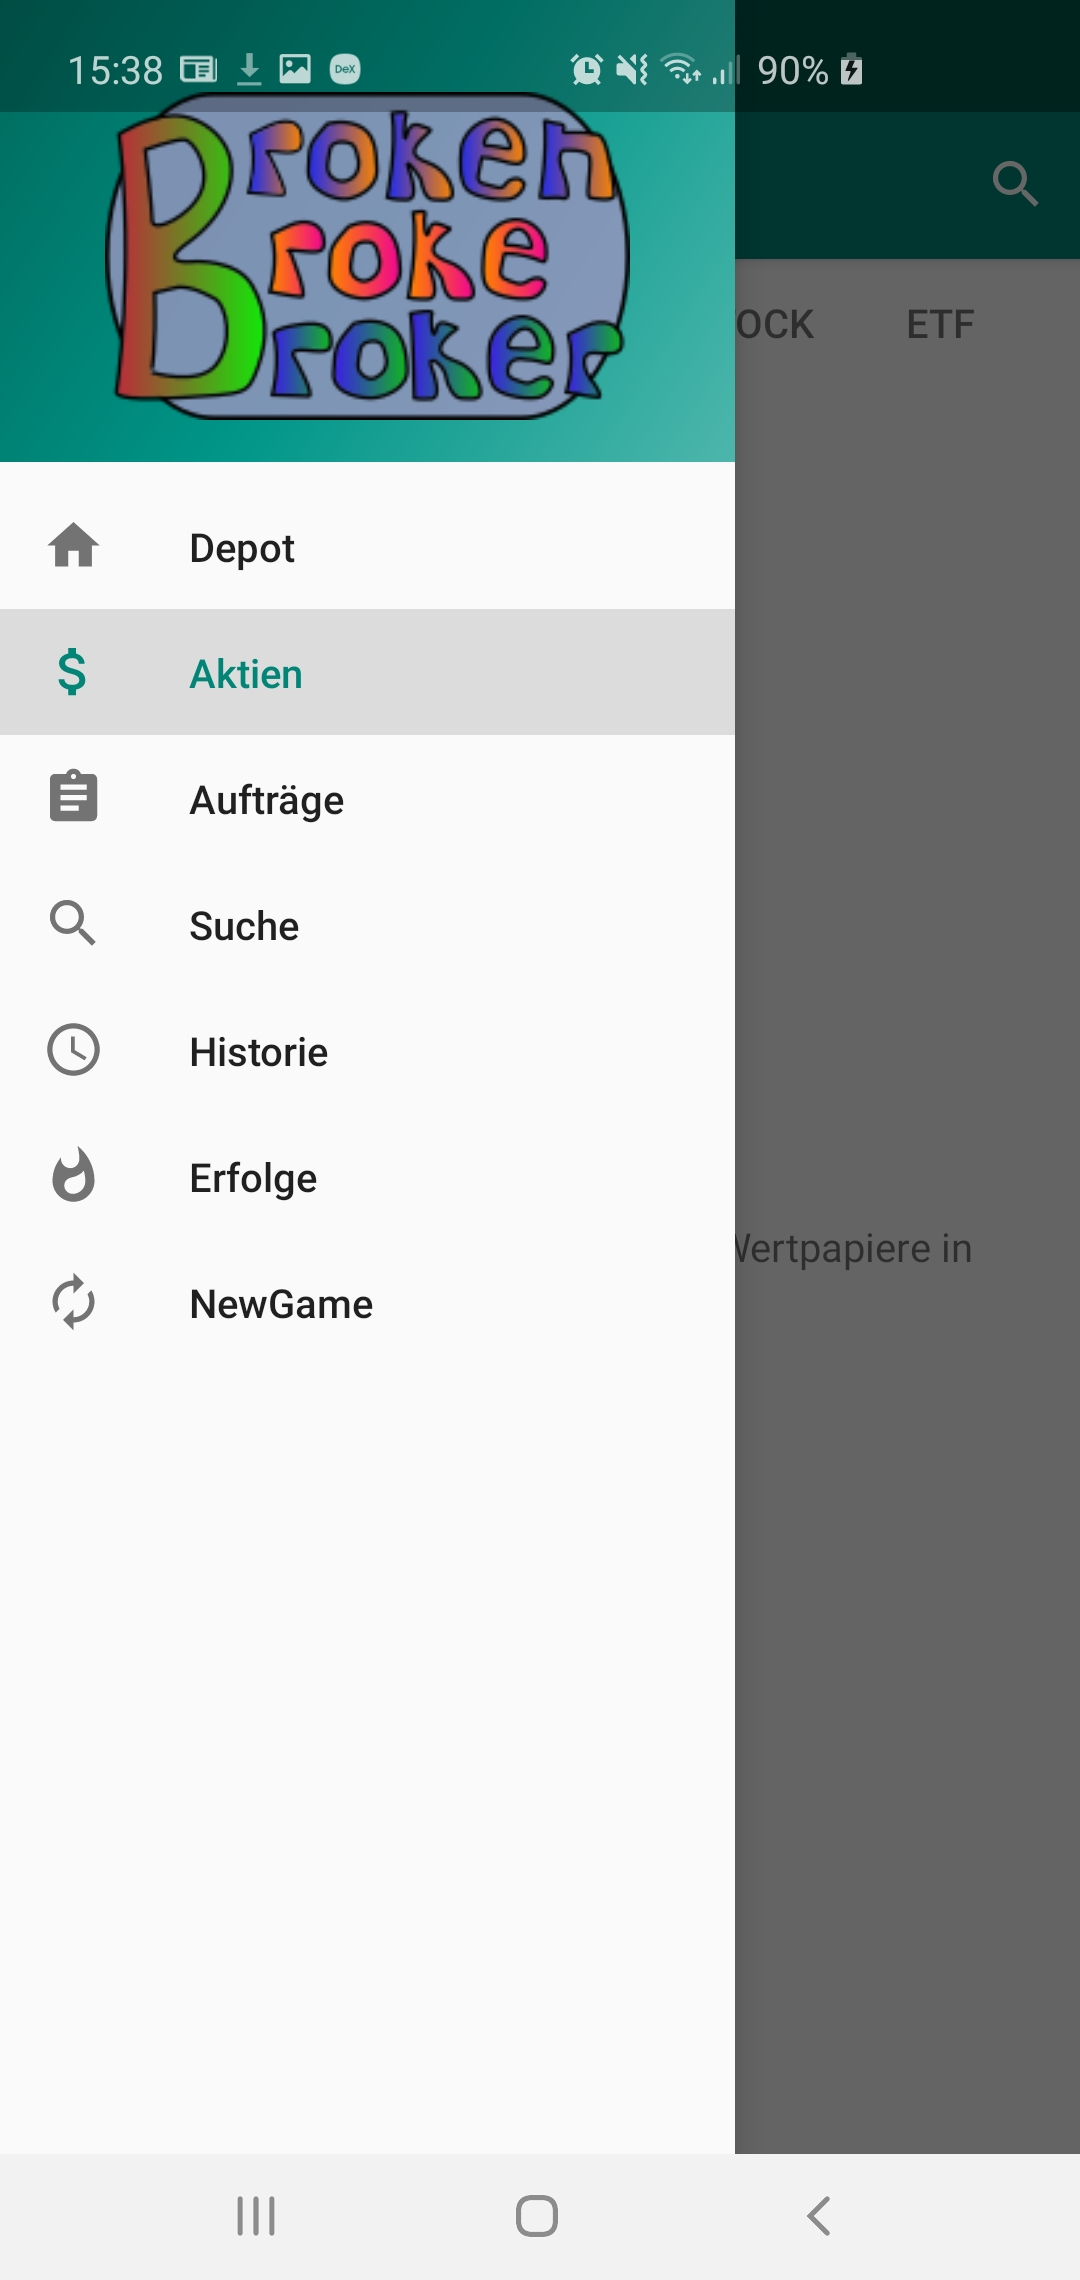
\includegraphics[width=0.6\textwidth]{Bilder/Applikation/Navigation.jpg}
\end{figure}

Bild der Navigation, die aktuelle Seite ist die, der markierten Reihe.

\begin{figure}[H]
	\centering
	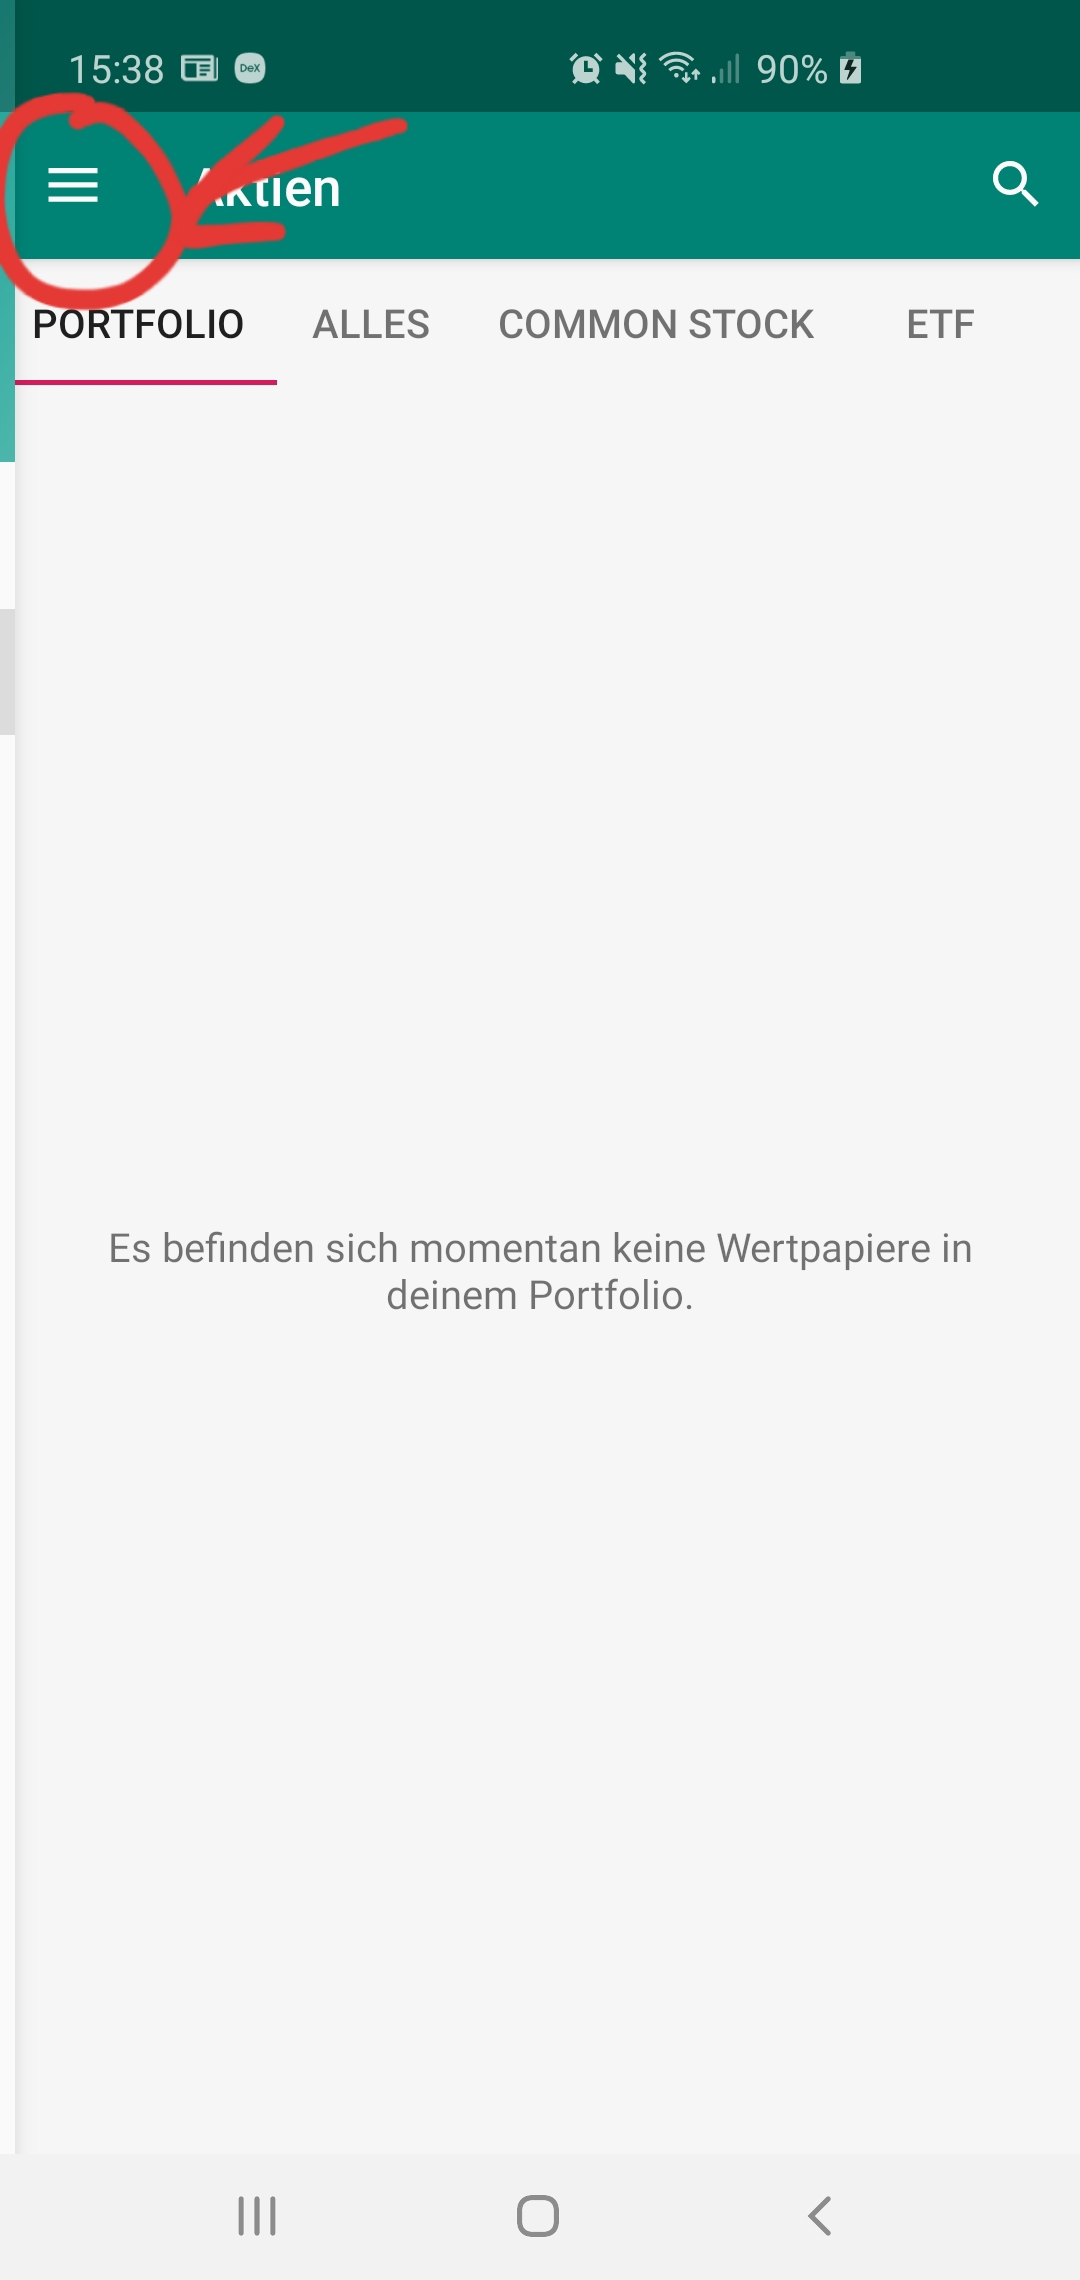
\includegraphics[width=0.6\textwidth]{Bilder/Applikation/NavigationsSymbol.jpg}
\end{figure}

Bild des Menüzeichens, mit dem sich die Navigation öffnen lässt. Die roten Striche zeigen auf das Symbol.

Hauptseite: Depot
Das Depot ist die erste Hauptseite und auch die Startseite. Nach dem Öffnen der Applikation gelangt man immer zu erst in der Depot, da sich das Spiel auch größtenteils um dessen Inhalt dreht. Dort werden nämlich die Hauptressourcen, die eigenen Aktion, verwaltet.
Das Depot ist eingeteilt in Übersicht und Statistik. Beide Punkte befinden sich nebeneinander direkt unterhalb der Leiste, die zur Navigation gehört. Der ausgewählte Punkt ist rot unterstrichen und beeinflusst den darunterliegenden Teil der Seite. Beim Start gelangt man immer zu Erst in die Übersicht aber wenn man sich beim letzten Verlassen der Seite in der Statistik befand, dann gelangt man beim nächsten Besuch auch zu erst in die Statistik. .
Die Übersicht beinhaltet als erstes den aktuellen Kontostand, sowie den gesamten Wert der Wertpapiere und die daraus resultierende Summe. Darunter sind dann die Wertpapiere, mit Menge und einzelnem Wert, aufgelistet. Geht die Liste nach unten hin über den Rand des Bildschirm hinaus, kann man die unteren Teile durch scrollen erreichen. Die oberen Listeneinträge werden dann durch die unteren ersetzt aber alles oberhalb der Liste bleibt unverändert.
\todo{Aktiendeteilansicht, beschreibung hier oder nur erwähnung?}
	
\todo{Bilder von Depot(Übersicht) einfügen}
	
	
\todo{Statistik, wenn fertig}

Hauptseite: Aktien
Wenn man das erste mal zu dieser Seite navigiert wird, gelangt man zu seinem Portfolio. Darin sind alle Aktien zu sehen, die man vorher zu dem Portfolio hinzugefügt hat. Es dient als eine Übersicht für die besonders interessanten Aktien, die man im Auge behalten möchte. Ähnlich wie bei Übersicht und Statistik im Depot befindet sich direkt unter der Navigationsleiste Wahlmöglichkeiten, die die Seite darunter verändern. Neben dem Portfolio gibt es dort die Möglichkeit auf "ALLES" zu klicken um eine Übersicht über alle verfügbaren Aktion zu bekommen. Die Leiste mit diesen Wahlmöglichkeiten lässt sich nach rechts scrollen, indem man die Leiste nach links zieht. Die weiteren Sektionen enthalten Teile von allen verfügbaren Aktien, die kategorisch zusammengefasst sind. Die Leiste enthält jedoch nicht alle möglichen Kategorien sondern nur diese, die auch Aktien enthalten. Die Liste wird regelmäßig geupdated, also ist es möglich, dass einige Kategorien aus der Leiste verschwinden oder hinzugefügt werden.
Durch klick auf eine bestimmte Aktie gelangt man zu der dazugehörigen Aktiendetailansicht. Der Knopf, der zur Navigation führt wird dann durch einen Pfeil ersetzt, der zurück zu der vorherigen Stelle in der Liste der Aktien führt.

Hauptseite: Aufträge

\todo{Aufträge, wenn fertig}

Hauptseite: Suche
Die Suche ist von Überall erreichbar, nicht nur, wenn man in der Navigation darauf klickt. Auf jeder Seite bindet sich am oberen Ende des Bildschirms eine Leiste, die zur Navigation gehört. Der rechte Teil enthält ein Suchsymbol, dass ein Textfeld in seine Leiste und eine Tastatur öffnet, wenn man darauf klickt. Mit der Tastatur kann man in das Textfeld schreiben und mit Enter seine Suche bestätigen. Durch diesen Prozess gelangt man zu der Hauptseite der Suche und die Aktien, die mit der Eingabe in Verbindung stehen, werden aufgelistet. Jeder Teil der aufgelisteten Aktien führt wieder zu der dazugehörigen Aktiendetailansicht. Über der Liste der Suchergebnisse steht unter anderem "Suchkategorie:". Rechts davon steht vom Anfang "ALLES" und noch weiter rechts davon ein kleines Dreieck mit der Spitze nach unten. Durch drücken auf den Teil zwischen dem Anfang von "ALLES" und dem Dreieck, fährt ein Menü aus, dass alle Kategorien der Suchergebnisse beinhaltet und die man durch Klick wählen kann. Die Liste wird daraufhin auf die Ergebnisse mit der gewählten Kategorie reduziert. Der Text "ALLES" wird durch den Namen der gewählten Kategorie ersetzt. 
Gelangt man durch den Eintrag in der Navigation zur Suche, so ist die Seite leer, wenn man vorher nichts gesucht hat. Hat man vorher allerdings schon mal etwas gesucht, so findet man die Seite in dem Zustand vor, wie man sie vorher verlassen hat.

\todo{Bilder von leerer und erfolgreicher Suche einfügen}

Hauptseite: Historie

Die Historie gibt einen Überblick über alle Käufe und Verkäufe von Aktien, sowie die Bilanz und aktuellen Besitz. Zu beginn des Spiels, bevor man irgendwelche Käufe oder Verkäufe durchgeführt hat, ist die Historie hoch leer und nur am unteren Ende des Bildschirms stehen Werte für Cash, Wertpapieren und die Bilanzsumme. Kauft oder Verkauft man nun jedoch Aktien, tauchen diese Aktionen von oben nach unten in der Reihenfolge der Ausführung auf. Die Einträge bestehen zu Erst aus entweder Plus oder Minus. Plus für Kauf, Minus für Verkauf der Aktien. Dahinter die Anzahl und ein "x" für Mal, und dann den Namen der Aktie. Darauf folgt dann eine freie Stelle, hinter der die Summe des Kauf- oder Verkaufspreises der einzelnen Aktien steht. Ganz rechts vom Eintrag befindet sich noch ein Dollarzeichen, dass zu dem Preis gehört.
Jeder Eintrag beeinflusst die darunterliegenden Werte von Cash, Wertpapieren und Bilanzsumme und diese passen sich entsprechend an.

Hauptseite: Erfolge

\todo{Erfolge, wenn fertig}

Hauptseite: NewGame

Die letzte Hauptseite "NewGame" gibt die Möglichkeit den Spielstand zurückzusetzen und von vorne zu beginnen. 
Auf der Seite steht nur die Frage, ob man sein Spiel wirklich neu beginnen möchte, der aktuelle Kontostand, den man damit zurücksetzt und ein roter Knopf mit dem Schriftzug "Zurücksetzen" darauf. Drückt man den Knopf, öffnet sich ein Popover, in dem man darauf hingewiesen wird, dass man damit auch alle Aktien im Besitz und die Favoriten löscht. Hier besteht noch die Möglichkeit auf "Abbruch" zu klicken. Drückt man nun jedoch auf "Ok", löschen sich alle spielstandrelevanten Daten. Man landet in einem leeren Depot aber kann direkt mit dem neuen Spielstand weiter spielen.

\subsection{Liste aller Klassen und deren Methoden mit Funktion}

\section{Klassendiagramm}

\subsection{Anbindung an das Datenmodell der API}

\subsection{Darstellung des Datenmodells als UML}

\subsection{Darstellung aller Views und deren Controller als UML}

\section{Überblick über die Umsetzung}
%Hier ist wichtig zu schreiben, was wir meinen Gut gemacht ist und wie dies mit den App zielen conquentiert.

\section{Fazit}
%Hier ist wichtig, dass wir es schaffen können zu zeigen, ob wir mit den erreichten Zielen zufrieden sind.





\end{document}